\chapter{Lineare Gleichungssysteme}

Problem: Finde $x \in \R^n$ so dass
\begin{equation*}
Ax = b
\end{equation*}
für gegebenes $A \in \R^{n\times n}$ und $b\in \R^n$.

\medskip

Dies ist ein \underline{sehr} wichtiges Problem!

\begin{enumerate}[1)]
\item Viele Anwendungsprobleme lassen sich in dieser Form schreiben
\item Die einzigen Gleichungssysteme, die sich tatsächlich direkt (d.h.\ nicht iterativ) lösen lassen
\item Nichtlineare Gleichungen werden häufig gelöst, indem Folgen von linearen Gleichungssystemen gelöst werden.
\end{enumerate}

\bigskip

\emph{Erinnerung:}
\begin{satz}
Es existiert ein eindeutiges $x \in \R^{n}$ mit $Ax = b$ genau dann wenn $\det A \neq 0$.
\end{satz}
Cramer'sche Regel: ($1750$, vorher schon Leibniz bekannt)
\begin{equation*}
x_i
=
\frac{\det A_i}{\det A}, \quad i = 1, \dots, n
\qquad
\text{wobei $A_i = A$ mit der $i$-ten Spalte durch $b$ ersetzt}
\end{equation*}

\medskip

Funktioniert, ist aber viel zu teuer!

\medskip

\begin{itemize}
\item $n+1$ Determinanten
\item $1$ Determinante: $\det A = \sum_{\sigma \in S_n} \operatorname{sgn}(\sigma) a_{1,\sigma(1)} \cdots a_{n,\sigma(n)}$
\item $n \cdot n!$ Multiplikationen (Es gibt auch schnellere Algorithmen)
\end{itemize}

\medskip

\begin{center}
\begin{tabular}{ r | r | r }
   $n$ & $(n+1)\cdot n \cdot n!$ & Zeit (bei $1$ GFLOP)\\
   \hline
  $1$ & $2$ & \\
  $2$ & $12$ & \\
  $3$ & $ 72$ & \\
  \hline
  $10$ & $400 \cdot 10^6$ & $0{,}4$\,s \\
  $11$ & $5{,}26 \cdot 10^9$ & $5{,}26$\,s \\
  $12$ & & $74$\,s\\
  $13$ & & $1133$s (ca.\ $19$ min)\\
  $14$ & & $5$\,h\\
  $15$ & & $87$\,h\\
  $16$ & & $65$ Tage\\
  $\vdots$ & $\vdots$&$\vdots$
\end{tabular}
\end{center}
Man könnte versucht sein, $A^{-1}$ zu berechnen und dann einfach
\begin{equation*}
x = A^{-1} b
\end{equation*}
zu setzen.
\\Davon ist abzuraten:
\begin{itemize}
\item Man löst quasi $Ax = b$ \underline{für alle $b$} 
\item Manchmal ist das schwierig, selbst wenn es für einzelne $b$ leicht ist.
\item Wenn man nur endliche Rechengenauigkeit hat wird $x$ möglicherweise sehr unpräzise.
\item Eine goldene Regel der Numerik:  Invertieren von Matrizen ist nie notwendig,
   und sollte immer vermieden werden.
\item Genaueres später
\end{itemize}

\section{Dreiecksmatrizen}
Das Lösen ist einfacher, wenn die Matrizen eine besondere Form haben.

\medskip

Ein wichtiger Fall: Dreiecksmatrizen
\begin{center}
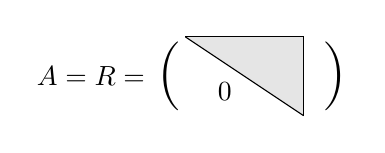
\begin{tikzpicture}[scale =2]
   \node (r0) at ( 0.0,  0.0) {};
   \node (s0) at (-0.75, 0.0) {};
   \node (s1) at ( 0.0, -0.5) {};
   \fill[fill=gray!20] (r0.center)--(s0.center)--(s1.center);
  \draw (-0.75,0) -- (0,0); \draw (-0.75,0) -- (0,-0.5); \draw (0,0) -- (0,-0.5);
  \draw (-0.5,-0.35) node {$0$};
  \draw (0.2,-0.25) node {\Huge{)}};
  \draw (-0.85,-0.25) node {\Huge{(}};
  \draw (-1.35, -0.25) node {$A = R =$};
\end{tikzpicture}
\begin{equation*}
Rx = z, \qquad r_{ij} =0, \quad i > j
\end{equation*}
\end{center}
\begin{align*}
 r_{11}x_1 + r_{12}x_2 + \dots + r_{1n}x_n & = z_1 \\
             r_{22}x_2 + \dots + r_{2n}x_n & = z_2 \\
                                           & \;\; \vdots \\
                                r_{nn}x_n  & = z_n
\end{align*}
Lösen durch \emph{Rückwärtssubstitution}:
\begin{align*}
x_n     & = z_n/ r_{nn} \\
x_{n-1} & = (z_n - r_{n-1,n}x_n)/ r_{n-1,n-1} \\
        & \; \; \vdots \\
x_1     & = (z_1 - r_{12}x_2 - \;\dots\; - r_{nn}x_n)/ r_{11}.
\end{align*}
Durchführbar, falls alle $r_{ii} \neq 0$, $i = 1, \dots, n$.
\begin{itemize}
\item Es gilt: $\det R = r_{11} \cdot r_{2} \cdots r_{nn}$
\item[$\Rightarrow$] Durchführbar, falls $\det R \neq 0$
\end{itemize}
Aufwand: $\approx \frac{n^2}{2}$ Multiplikationen/Divisionen

\section{Das Gaußsche Eliminationsverfahren}

\begin{itemize}
\item Von Gauß $1809$ beschrieben (als bekannt erwähnt!)
\item Lagrange schon $1759$ bekannt
\item In China schon kurz vor Christi Geburt bekannt 
\end{itemize}
Allgemeines Gleichungssystem:
\begin{equation*}
Ax =b
\end{equation*}
Ausgeschrieben:
\begin{center}
\begin{tabular}{ c c c c c c c l }
$a_{11}x_1 $&$+$ & $ a_{12}x_2 $&$+ $ & $\dots$ & $+ $&$a_{1n}x_n \; =$ &  $b_1$
\\ $a_{21}x_1 $&$+$ & $ a_{22}x_2 $&$+ $ & $\dots$ & $+ $&$a_{2n}x_n \; =$ &  $b_2$
\\ $\vdots$&&$\vdots$&&&&$\vdots$&$\vdots$
\\ $a_{n1}x_1 $&$+$ & $ a_{n2}x_2 $&$+ $ & $\dots$ & $+ $&$a_{nn}x_n \; =$ &  $b_n$
\end{tabular}
\end{center}
\underline{Idee:} Forme Gleichungssystem in ein oberes Dreieckssystem um.

\medskip

Dafür ausreichend: eliminere alle Einträge unterhalb von $a_{11}$ (der Rest geht rekursiv).

\medskip

Wie macht man das?
\begin{itemize}
\item Voraussetzung: $a_{11} \neq 0$
\item Um $a_{i1}x_1$ in Zeile $i$, ($i = 2, \dots, n$) zu eliminieren:
\item[$\rightarrow$] Subtrahiere von Zeile $i$ ein Vielfaches von Zeile $1$
\end{itemize}
Neue Zeile $i$:
\begin{equation*}
\underbrace{(a_{i1} - l_{i1}a_{11})}_{\substack{= \; 0 \\ \textnormal{falls } l_{i1} = \frac{a_{i1}}{a_{11}}}} x_1 + \underbrace{(a_{i2} - l_{i1}a_{12})}_{\equalscolon a'_{i2}} x_2 + \dots +
\underbrace{(a_{in} - l_{i1}a_{1n})}_{\equalscolon a'_{in}} x_n =
\underbrace{b_i - l_{i1}b_1}_{\equalscolon b'_i}
\end{equation*}
\begin{itemize}
\item Durchführbar falls $a_{11} \neq 0$.
\item In den Zeilen $2, \dots, n$ steht eine $(n-1) \times (n-1)$-Matrix
\item Man wende das Verfahren darauf an:
\item[$\Rightarrow$] Folge von Matrizen:
\begin{equation*}
A = A^{(1)} \rightarrow A^{(2)} \rightarrow A^{(n)} \equalscolon R
\end{equation*}
\end{itemize}
Wir haben das allgemeine Gleichungssystem $Ax = b$ in ein Dreieckssystem $Rx = z$ umgeformt.

\subsection{Aufwand}

\begin{itemize}
\item Rechenaufwand für die Umformung: $O(n^3)$ Multiplikationen
\item Lösen des Dreieckssystems: $O(n^2)$ Schritte
\item[$\rightarrow$] insgesamt also $O(n^3)$
\\ Immer noch viel, aber deutlich besser als $(n+1)\cdot n\cdot n!$
\end{itemize}

Laufzeit:

\begin{tabular}{ r | r | r }
  $n$ & $n^3$ & Zeit bei 1~GFLOP\\ \hline
  $1$ & $1$ \\
  $2$ & $8$ \\
  $3$ & $27$ \\
  $10$ & $1000$ \\
  $100$ & $1\cdot 10^6$ \\
  $1000$ & $1\cdot 10^9$ & $1s$
\end{tabular}

\section{Durchführbarkeit}
Vorwärtselimination ist durchführbar, falls $a_{kk}^{(k)} \neq 0$, $k = 1, \dots n$.

\medskip

\emph{Problem:} Diese Zahlen entstehen erst während des Verfahrens.

\medskip

Entscheide a priori, ob das Gauß-Verfahren für ein $A$ durchführbar ist.
\begin{definition}
Eine Matrix $A = (a_{ij}) \in \R^{n\times n}$ heißt streng diagonaldominant, falls
\begin{equation*}
\vert a_{ii} \vert > \sum_{\substack{j=1 \\ j \neq i}}^n \vert a_{ij} \vert \textnormal{ für alle } i = 1, \dots, n
\end{equation*}
\end{definition}

\begin{lemma}
Falls $A \in \R^{n \times n}$ streng diagonaldominant ist, so ist die Vorwärtselimination durchführbar.
\end{lemma}
\begin{proof}
Die Matrix $A^{(1)}$ ist streng diagonaldominant.
\begin{itemize}
\item[$\rightarrow$] Also insbesondere $\vert a_{11} \vert > 0$
\item[$\rightarrow$] Der erste Schritt ist durchführbar.
\end{itemize}
Induktion: Aus $A^{(k)}$ streng diagonaldominant folgt $A^{(k+1)}$ streng diagonaldominant.
\begin{itemize}
\item Sei $i$ eine Matrixzeile.
\item Falls $i \le k$, so ist die $i$-te Zeile  von $A^{(k+1)}$ identisch mit der $i$-ten Zeile von $A^{(k)} \\
   \rightarrow$ nichts zu zeigen.
\item Sei also $i > k$.
\end{itemize}
\begin{align*}
\sum_{\substack{j = 1 \\ j \neq i}}^{n} \Big\vert a_{ij}^{(k+1)}\Big\vert & = \sum_{\substack{j = k+1 \\ j \neq i}}^{n} \Big\vert a_{ij}^{(k+1)}\Big\vert
\qquad \text{(für kleinere $j$ ist $a_{ij}^{(k+1)} = 0$)} \\
%
& =
\sum_{\substack{j = k+1 \\ j \neq i}}^{n}  \Bigg\vert a_{ij}^{(k)} - \frac{a_{kj}^{(k)}a_{ik}^{(k)}}{a_{kk}^{(k)}}\Bigg\vert
\qquad
\text{($k+1$-ter Eliminationsschritt)} \\
%
& \le
\sum_{\substack{j = k+1 \\ j \neq i}}^{n} \Big\vert a_{ij}^{(k)} \Big\vert + \Bigg\vert \frac{a_{ik}^{(k)}}{a_{kk}^{(k)}}\Bigg\vert \;\sum_{\substack{j = k+1 \\ j \neq i}}^{n} \Big\vert a_{kj}^{(k)} \Big\vert \\
%
& = \underbrace{\sum_{\substack{j = k \\ j \neq i}}^{n} \Big\vert a_{ij}^{(k)} \Big\vert}_{< \vert a_{ii}^{(k)} \vert}
- \Big\vert a_{ik}^{(k)} \Big\vert
  +
  \Bigg\vert \frac{a_{ik}^{(k)}}{a_{kk}^{(k)}} \Bigg\vert
  \Bigg(\underbrace{\sum_{j = k+1}^{n} \Big\vert a_{kj}^{(k)} \Big\vert}_{< \vert a_{kk}^{(k)} \vert}
-\Big\vert a_{ki}^{(k)} \Big\vert \Bigg)
\\ & < \Big \vert a_{ii}^{(k)} \Big\vert - \cancel{\Big \vert a_{ik}^{(k)} \Big\vert} + \Bigg\vert \frac{a_{ik}^{(k)}}{a_{kk}^{(k)}}\Bigg\vert \Bigg(\cancel{\Big\vert a_{kk}^{(k)} \Big\vert}
-\Big\vert a_{ki}^{(k)} \Big\vert \Bigg)
\\ & = \Big \vert a_{ii}^{(k)} \Big\vert - \Bigg\vert \frac{a_{ik}^{(k)} a_{ki}^{(k)}}{a_{kk}^{(k)}}\Bigg\vert
\\ & \le \Bigg\vert a_{ii}^{(k)} - \frac{a_{ik}^{(k)} a_{ki}^{(k)}}{a_{kk}^{(k)}}\Bigg\vert
\\ & = \Big\vert a_{ii}^{(k+1)}\Big\vert.
\qedhere
\end{align*}
\end{proof}
\begin{kor} Sei $A$ streng diagonaldominant. Dann ist auch die Rückwärtssubstitution durchführbar.
\end{kor}
\begin{proof}
$R = A^{(n)}$ ist streng diagonaldominant, also sind alle Diagonalelemente $\neq 0$.
\end{proof}

\section{Die LR-Zerlegung}

Folge von Matrizen:
\begin{equation*}
A = A^{(1)} \rightarrow A^{(2)} \rightarrow A^{(n)} \colonequals R
\end{equation*}
Der Übergang von $A^{(k)}, b^{(k)}$ zu $A^{(k+1)}, b^{(k+1)}$ ist \underline{linear}
\medskip

\qquad $\Rightarrow$ Es gibt eine Matrix $L_k \in \R^{n \times n}$, so dass
\begin{equation*}
A^{(k+1)} = L_k A^{(k)}
\qquad \text{und} \qquad
b^{(k+1)} = L_k b^{(k)}.
\end{equation*}
Die Matrix $L_k$ heißt \emph{Frobenius-Matrix}.
\begin{itemize}
\item Explizite Form:
\begin{equation*}
L_k = \begin{pmatrix}
1 & & & & &
\\ & \ddots & & & &
\\ & & 1 & & &
\\ & & -l_{k+1, k} & 1 & &
\\ & & \vdots & & \ddots &
\\ & & -l_{n,k} & & & 1
\end{pmatrix}
\end{equation*}
\item Interessanterweise:
\begin{equation*}
L_k^{-1} = \begin{pmatrix}
1 & & & & &
\\ & \ddots & & & &
\\ & & 1 & & &
\\ & & l_{k+1, k} & 1 & &
\\ & & \vdots & & \ddots &
\\ & & l_{n,k} & & & 1
\end{pmatrix}
\end{equation*}
\item Außerdem:
\begin{equation*}
L^{-1} \colonequals L_{n-1} \cdots L_{n-2} \cdot \dots \cdot L_1= \begin{pmatrix}
1 & & & &
\\ -l_{21}& 1 & & &
\\ -l_{31}& -l_{32} & 1& &
\\ \vdots & & & \ddots &
\\ -l_{n1} & & & -l_{n, n-1} & 1
\end{pmatrix}
\end{equation*}
\end{itemize}

Damit ist
\begin{equation*}
R = A^{(n)} = L_{n-1}A^{(n-1)} = L_{n-1}L_{n-2}A^{(n-2)} = L^{-1}A^{(1)} = L^{-1}A,
\end{equation*}
also
\begin{equation*}
A= LR
\qquad \text{und} \qquad
z = L^{-1}b.
\end{equation*}
Diese Zerlegung von $A$ in zwei Dreiecksmatrizen heißt \emph{$LR$-Zerlegung}.

\medskip

(Häufig auch $LU$-Zerlegung, wegen englisch: ``lower-upper'')

\bigskip

Die Gauß-Elimination nimmt damit folgende Form an:
\begin{enumerate}[1)]
\item Berechne Zerlegung $A= LR$
\item Bestimme $z \in \R^n$ so dass $Lz =b$ (Vorwärtssubstitution)
\item Bestimme $x \in \R^n$ so dass $Rx = z$ (Rückwärtssubstitution)
\end{enumerate}
Vorteil dieser Sichtweise: nur $1)$ ist teuer $(O(n^3))$, Schritte $2)$ und $3)$ sind in $O(n^2)$.
\begin{itemize}
\item Falls man mehrere Gleichungssysteme $Ax_i = b_i$, $i = 1, \dots, m$ zu lösen hat, muss man den teuren Schritt $1)$ nur einmal machen.
\end{itemize}

\begin{bem}
Die $LR$-Zerlegung bietet auch eine klassische Möglichkeit, um die Determinante von $A$ auszurechnen.
Denn
\begin{align*}
 \det A & = \det LR = \det L \cdot \det R
          = \prod_{i=1}^n \underbrace{l_{ii}}_{=1} \cdot \prod_{i=1}^n r_{ii}
          = \prod_{i=1}^n r_{ii}.
\end{align*}

\end{bem}


\section{Pivot-Strategien}

Die Elemente der Matrizen $A^{(k)}$ durch die dividiert wird nennt man \emph{Pivot-Elemente}
(Pivot: frz.: Drehpunkt)

\subsection{Probleme mit der einfachen Gauß-Elimination}

Es ist einfach, Fälle zu konstruieren, wo Gauß-Elimination versagt, z.\,B.
\begin{equation*}
A =
\begin{pmatrix}
0 & 1 \\
1 & 0
\end{pmatrix},
\qquad
\det A = -1 \neq 0.
\end{equation*}
$\rightarrow$ Lösung: vertausche einfach die beiden Zeilen!

\bigskip

Bevor wir diese Idee formalisieren:
\\$\rightarrow$ Das Problem ist noch schlimmer:

\medskip

Auch Pivot-Elemente, die $\neq 0$, aber sehr klein sind machen Probleme.
\begin{bsp}
\begin{align*}
10^{-4} x_1 + x_2 & = 1 \\
        x_1 + x_2 & = 2
\end{align*}

\medskip

Zum Lösen eliminieren wir $a_{21}$:

Die zweite Zeile wird:
\begin{equation*}
0 - 9999x_2 = -9998
\end{equation*}
Rückwärtssubstitution:
\begin{align*}
x_2 & = \frac{9998}{9999} = 0{,}\overline{9998} \\
%
x_1 & = 10000(1-x_2) = 10000\Big(\frac{1}{9999}\Big) = 1{,}\overline{0001}.
\end{align*}
\emph{Realität:} Rechner können nur Zahlen mit einer Maximalzahl an Dezimalstellen
darstellen.

\medskip

Beispiel: 3 Dezimalstellen

\medskip

Runden der exakten Lösung auf $3$ Stellen: $x_1 = 1, x_2 = 1$.

\medskip

Dieses Ergebnis würden wir erwarten. Aber\dots
\bigskip

Jetzt machen wir Gauß-Elimination und haben zu jedem Zeitpunkt nur 3 gültige Stellen:
\begin{align*}
1{,}00 \cdot 10^{-4} x_1 + 1{,}00x_2 & = 1{,}00 \\
1{,}00 x_1 + 1{,}00x_2 & = 2{,}00
\end{align*}
Eliminiere die zweite Zeile.  Dafür brauchen wir den Faktor
\begin{equation*}
l_{21} = \frac{1{,}00}{1{,}00 \cdot 10^{-4}} = 1{,}00 \cdot 10^4
\end{equation*}
Aus der zweiten Zeilen wird:
\begin{equation*}
\big(1{,}00 - 1{,}00\cdot 10^4 \cdot 1{,}00 \cdot 10^{-4}\big)x_1
    + \big( 1{,}00 - 1{,}00 \cdot 10^4 \cdot 1{,}00 \big) x_2
 =
 2{,}00 - 1{,}00\cdot 10^4 \cdot 1{,}00
\end{equation*}
bzw.
\begin{align*}
0 \cdot x_1 + \underbrace{\Big( 1{,}00 - 10000\Big)}x_2 & = 2{,}00 - 10\,000
\\ -9\,990 \hspace{2.2em}x_2 &= - 9\,990
\end{align*}
Rückwärtssubstitution:
\begin{align*}
 x_2 & = 1{,}00 \qquad \checkmark \\
 x_1 & = 0 \hspace{1em} \qquad  \frownie
\end{align*}
\end{bsp}

Der Algorithmus hat anscheinend ein völlig falsches Ergebnis produziert!

\bigskip

Fazit: Das Gauß-Verfahren versagt
\begin{enumerate}[a)]
 \item falls eins der Pivotelemente $a_{kk}^{(k)}$ gleich Null ist.
 \item Anscheinend versagt es zumindest manchmal auch, wenn $a_{kk}^{(k)} \neq 0$ aber klein ist,
 und wir nur eine endliche Rechengenauigkeit haben (so richtig verstanden haben wir das noch nicht).
\end{enumerate}

\subsection{Pivot-Strategien}

Als $a_{11} = 0$ war hat Vertauschen der Zeilen geholfen.

\medskip

Das probieren wir jetzt noch mal:

\begin{align*}
1{,}00 x_1 + 1{,}00x_2 & = 2{,}00 \\
1{,}00 \cdot 10^{-4} x_1 + 1{,}00x_2 & = 1{,}00
\end{align*}

Faktor zum Eliminieren von $\tilde{a}_{21}$:
\begin{equation*}
 \tilde{l}_{21} = 1{,}00 \cdot 10^{-4}.
\end{equation*}
Dreiecksystem:
\begin{align*}
1{,}00 x_1 + 1{,}00x_2 & = 2{,}00 \\
 1{,}00x_2 & = 1{,}00
\end{align*}
Rückwärtssubstitution:
\begin{equation*}
 x_2 = 1{,}00,
 \qquad
 x_1 = 1{,}00
\end{equation*}

Warum hat das besser funktioniert?
\begin{equation*}
 \abs{\tilde{l}_{21}} < 1
 \qquad \text{bzw.} \qquad
 \abs{\tilde{a}_{11}} \ge \abs{\tilde{a}_{21}}
\end{equation*}



\bigskip

\paragraph{Idee der Spaltenpivotisierung:}
\begin{itemize}
\item Vertausche Zeilen(!) der Matrix, um ein möglichst geeignetes Pivot-Element zu finden.
\end{itemize}
Algorithmus:
\begin{enumerate}[a)]
\item Wähle im Schritt $A^{(k)} \rightarrow A^{(k+1)}$ ein $p \in \{ k, \dots, n \}$ so dass
\begin{equation*}
\Big\vert a_{pk}^{(k)} \Big\vert \ge \Big\vert a_{jk}^{(k)} \Big\vert
\qquad
\forall j = k, \dots, n.
\end{equation*}
\item Vertausche die Zeilen $p$ und $k$
\begin{equation*}
A^{(k)} \rightarrow \tilde{A}^{(k)}
\qquad \text{mit} \qquad
\tilde{a}_{ij}^{(k)} =
\begin{cases}
a_{kj}^{(k)} & \text{falls $i = p$} \\
a_{pj}^{(k)} & \text{falls $i = k$} \\
a_{ij}^{(k)} & \text{sonst}.
\end{cases}
\end{equation*}
Es gilt immer $\displaystyle \vert \tilde{l}_{ik} \vert = \bigg\vert \frac{\tilde{a}_{ik}^{(k)}}{\tilde{a}_{kk}^{(k)}}\bigg\vert = \bigg\vert \frac{a_{ik}^{(k)}}{a_{pk}^{(k)}}\bigg\vert \le 1$
\item Führe den nächsten Eliminationsschritt mit $\tilde{A}^{(k)}$ statt $A^{(k)}$ aus:
\begin{equation*}
\tilde{A}^{(k)} \rightarrow A^{(k+1)}.
\end{equation*}
\end{enumerate}

\begin{satz}[\citeauthor{deuflhard_hohmann:1993}, Satz~1.8]
Falls $A$ nicht singulär ist, so ist die Gauß-Elimination mit Spaltenpivotisierung durchführbar.
\end{satz}
Zusätzlicher Aufwand: $O(n^2)$

Es gibt auch:
\begin{itemize}
\item Zeilenpivotisierung $\rightarrow$ vertausche Spalten
\item vollständige Pivotisierung: vertausche Zeilen \underline{und} Spalten
\\Aufwand: $O(n^3)$, wird nur sehr selten verwendet.
\end{itemize}



\section{Nachiteration}

(engl.\ \emph{iterative refinement})

\bigskip

Selbst mit Pivotisierung kann die Lösung noch ziemlich ungenau sein.

\bigskip

\paragraph{Idee der Nachiteration:}

\begin{itemize}
 \item Sei $x$ die exakte Lösung.
 \item Sei $\tilde{x}$ die numerische Lösung.
 \item Der Fehler $\delta \colonequals x - \tilde{x}$ löst die \emph{Defektgleichung}
  \begin{equation}
  \label{eq:lineare_gleichungssysteme:defektgleichung}
   A \delta = r(\tilde{x}) \colonequals b - A \tilde{x}
  \end{equation}

 \item Löse dieses System numerisch.  Nenne die Lösung $\tilde{\delta}$.
 \item Dann ist $\tilde{x} + \tilde{\delta}$ eine bessere Lösung des Ausgangsproblems
   als $\tilde{x}$.
 \item Falls nötig: Wiederholen.
 \item Lösen von \eqref{eq:lineare_gleichungssysteme:defektgleichung} kostet nur $O(n^2)$
  Operationen, da die Zerlegung der Matrix $A$ wiederverwendet werden kann.

\end{itemize}

